\subsection{SUMO}
\label{sec:sumo}

SUMO (Simulation Of Urban Mobility) is a free and open-source traffic microsimulator. It provides interactive graphical tools for both visualising simulations and creating road networks. Real-world networks can also be imported from Open Street Map \cite{haklay2008openstreetmap}. SUMO allows intermodal traffic simulation by modelling pedestrians, public transport and cyclists.

In \cite{kotusevski2009review} the authors show that SUMO begins to suffer from performance degradation when simulations exceed 10,000 road network edges, while macrosimulators can cope with very large networks without any performance issues. Our goal is to show that emulation using Gaussian Processes (GPs) can enable users to obtain the detailed output of microsimulations by querying an easy-to-compute surrogate model, preventing them from falling back to less detailed macrosimulation models due to scalability issues.

\subsection{Map Creation}
\label{sec:map_creation}

We study the traffic congestion problem in the context of cities. In order to be able to tune different road network parameters programmatically, custom networks are generated with a lattice grid topology as seen in Figure~\ref{fig:custom_network}. These networks represent a portion of a city or a district. Grids have been chosen since ancient Roman times as the main topology for urban environments and, still today, characterise the outline of many major cities in the world (e.g., New York).

\begin{figure}[b!]
    \centering
    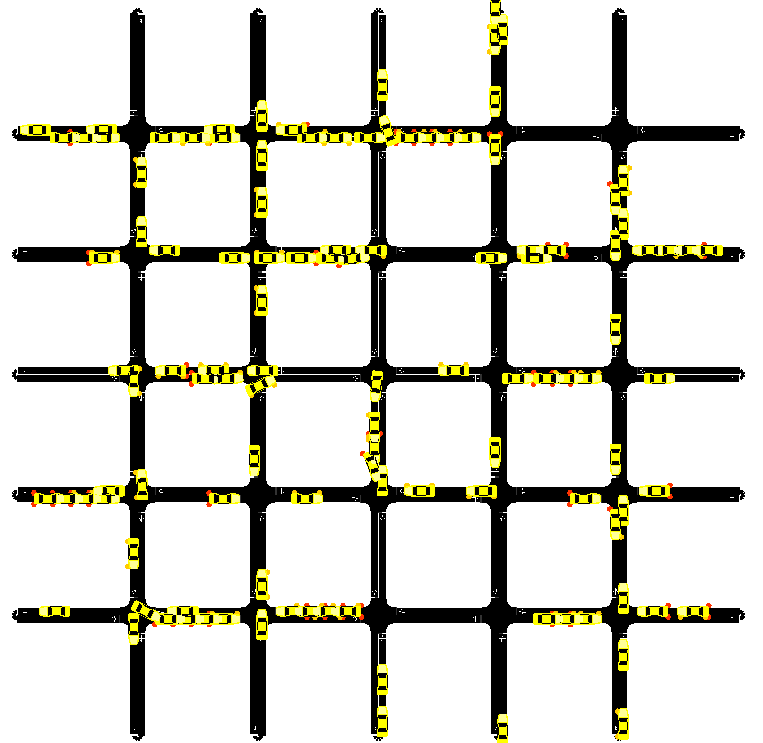
\includegraphics[width=0.4\textwidth]{custom_net}
    \caption{Custom generated $5\times5$ grid network}
    \label{fig:custom_network}
\end{figure}


\begin{table}[h!]
    \centering
    \caption{Tunable parameters of the custom grid network}
    \label{table:grid_params}
    \begin{tabular}{@{} l *4c @{}}
    \toprule
     \multicolumn{1}{c}{Parameter name} & Description \\ 
    \midrule
    Grid Size ($N_G$) & Number of intersections along a single axis of the grid \\ 
    Junction Type & How traffic is regulated at intersections \\ 
    Edge Length ($L_E$) & The distance between two intersections in meters\\
    Number of Lanes ($N_L$) & The number of lanes of each road \\
    Edge Max Speed ($v_{max}$) & The speed limit in the network \\
    \bottomrule
    \end{tabular}
\end{table}

The grids created for our simulation present the parameters shown in Table \ref{table:grid_params}. Intersections are regulated by actuated traffic lights\footnote{Green phases may be prolonged depending on traffic measurements from automatically added induction loops}. Grid size ($N_G$), edge length ($L_E$), and number of lanes ($N_L$) are the parameters that we are interested in varying throughout our simulations.


\subsection{Route Planning}
\label{sec:trip_generation}

In order to simulate traffic flow in the generated network, vehicles' trips that resemble real urban traffic were generated. For this purpose, we used the \verb|randomTrips| tool provided by SUMO, which is able to generate random trips given an input road network, vehicle specification and route properties. This tool automatically ensures that routes and networks are valid. 

\begin{table}[h!]
    \centering
    \caption{Tunable parameters of the vehicle generator}
    \label{table:veh_params}
    \begin{tabular}{@{} l *4c @{}}
        \toprule
        \multicolumn{1}{c}{Parameter name} & Description \\ 
        \midrule
        Vehicle Class  & Vehicle type eg. passenger, emergency, bus \\
        Emissions Class  & Vehicle emissions as per the HBEFA v3.1 standard \\
        Acceleration ($\alpha_V$)  & Maximum vehicle acceleration \\
        Deceleration  & Maximum vehicle deceleration \\
        Max Speed  & Maximum vehicle speed \\
        Speed Factor  & Expected multiplier for lane speed limits \\
        Speed Deviation  & The deviation of the speed factor \\
         \bottomrule
    \end{tabular}
\end{table}

The generator creates vehicles with the properties seen in Table~\ref{table:veh_params}. This allows many different vehicle types to be explored, however, to reduce emulator complexity, only passenger vehicles are generated. Every vehicle has the emission class of a gasoline-driven passenger car (Euro norm 4 HBEFA v3.1-based). Additionally, the maximum deceleration remains constant at $4.5~m/s^2$, the speed factor equals $1$ with a $0.1$ random deviation.

\begin{table}[h!]
    \centering
    \caption{Tunable parameters of the trip generator}
    \label{table:trip_params}
    \begin{tabular}{@{} l *4c @{}}
        \toprule
        \multicolumn{1}{c}{Parameter name} & Description \\ 
        \midrule
        Begin Time ($t_b$)  & Trip departure begin time\\
        End Time ($t_e$)  & Trip departure end time \\
        Period ($\Delta t_V$) & Vehicle departure period \\
        Fringe Factor & Probability multiplier for trips to start on the edge of the network  \\
        \bottomrule
    \end{tabular}
\end{table}

Once the vehicle has been created, trips are generated on the road grid. These trips can be tuned using the parameters seen in Table~\ref{table:trip_params}. Trips depart throughout the simulation time, which has a duration of $300~s$. In order to simulate a grid which is part of a larger network, vehicles are 10 times more likely to start or end their trip on the edge of the network. This is set by the fringe factor. 

\subsection{Tuning congestion}
\label{sec:tuning_congestion}

The shape of the simulated networks varies greatly between different simulations. This is because it is highly dependent on the $N_G$ and $L_E$. Therefore, if we generate the same number of vehicles $N_V$ for every network we will obtain unbalanced traffic congestion throughout the simulations. Small grids are highly congested while large ones have free-flowing traffic. 

In order to keep traffic flow constant between different simulations, we start by defining the total number of roads in the grid $N_{roads}$ and the total number of road meters in the grid $L_{roads}$.

\begin{equation}
    N_{roads} = 2 N_G (N_G - 1) + 4 N_G
\end{equation} 
\begin{equation}
    L_{roads} = N_{roads} L_E
\end{equation}

The maximum number of vehicles $N_{V_{max}}$ that is possible to fit in the simulation will then be:

\begin{equation}
    N_{V_{max}} = \frac{L_{roads}}{\text{Vehicle Length}}
\end{equation}

Finally, to achieve constant traffic density, in each simulation we generate only a percentage of this number by multiplying it by a scaling factor $\beta$. We choose a value of 0.05 for $\beta$ which allows a moderate degree of traffic congestion while avoiding grid-lock.

\begin{equation}
    N_V = \beta  N_{V_{max}}
\end{equation}

Equation~\ref{eqn:num_cars} is used to set the vehicle generation period of the simulation.

\begin{equation}\label{eqn:num_cars}
   \Delta t_V  = \frac{t_e  - t_b}{N_V}
\end{equation}